\documentclass[11pt]{article}
\usepackage{lmodern}
\usepackage{amssymb,amsmath}
\usepackage{ifxetex,ifluatex}
\usepackage{fixltx2e} % provides \textsubscript
\ifnum 0\ifxetex 1\fi\ifluatex 1\fi=0 % if pdftex
  \usepackage[T1]{fontenc}
  \usepackage[utf8]{inputenc}
\else % if luatex or xelatex
  \ifxetex
    \usepackage{mathspec}
    \usepackage{xltxtra,xunicode}
  \else
    \usepackage{fontspec}
  \fi
  \defaultfontfeatures{Mapping=tex-text,Scale=MatchLowercase}
  \newcommand{\euro}{€}
\fi
% use upquote if available, for straight quotes in verbatim environments
\IfFileExists{upquote.sty}{\usepackage{upquote}}{}
% use microtype if available
\IfFileExists{microtype.sty}{%
\usepackage{microtype}
\UseMicrotypeSet[protrusion]{basicmath} % disable protrusion for tt fonts
}{}
\ifxetex
  \usepackage[setpagesize=false, % page size defined by xetex
              unicode=false, % unicode breaks when used with xetex
              xetex]{hyperref}
\else
  \usepackage[unicode=true]{hyperref}
\fi
\usepackage[usenames,dvipsnames]{color}
\hypersetup{breaklinks=true,
            bookmarks=true,
            pdfauthor={},
            pdftitle={},
            colorlinks=true,
            citecolor=blue,
            urlcolor=blue,
            linkcolor=magenta,
            pdfborder={0 0 0}}
\urlstyle{same}  % don't use monospace font for urls
\usepackage{longtable,booktabs}
\usepackage{graphicx,grffile}
\makeatletter
\def\maxwidth{\ifdim\Gin@nat@width>\linewidth\linewidth\else\Gin@nat@width\fi}
\def\maxheight{\ifdim\Gin@nat@height>\textheight\textheight\else\Gin@nat@height\fi}
\makeatother
% Scale images if necessary, so that they will not overflow the page
% margins by default, and it is still possible to overwrite the defaults
% using explicit options in \includegraphics[width, height, ...]{}
\setkeys{Gin}{width=\maxwidth,height=\maxheight,keepaspectratio}
\setlength{\parindent}{0pt}
\setlength{\parskip}{6pt plus 2pt minus 1pt}
\setlength{\emergencystretch}{3em}  % prevent overfull lines
\providecommand{\tightlist}{%
  \setlength{\itemsep}{0pt}\setlength{\parskip}{0pt}}
\setcounter{secnumdepth}{0}

\date{}

% Redefines (sub)paragraphs to behave more like sections
\ifx\paragraph\undefined\else
\let\oldparagraph\paragraph
\renewcommand{\paragraph}[1]{\oldparagraph{#1}\mbox{}}
\fi
\ifx\subparagraph\undefined\else
\let\oldsubparagraph\subparagraph
\renewcommand{\subparagraph}[1]{\oldsubparagraph{#1}\mbox{}}
\fi

\setlength{\oddsidemargin}{-0.1in}
\setlength{\topmargin}{-0.52truein} 
\setlength{\textheight}{9.15in} 
\setlength{\textwidth}{6.7in}

\usepackage[T1]{fontenc}
\usepackage{fourier}
\usepackage[sc]{mathpazo}
\linespread{1.05}         % Palatino needs more leading (space between lines)


\usepackage{wrapfig}
\usepackage[square,numbers,sort&compress]{natbib}
\renewcommand{\cite}{\citep}
%\usepackage[psamsfonts]{amssymb}
%\usepackage{palatino}
%\usepackage{mathpazo}

%\usepackage{plasmadefs}

\hyphenation{wave-packet wave-packets}

\title{}

\begin{document}

\section{Equipment}
The following subsections list the major items of equipment currently available for users of the Basic Plasma Science Facility.

\subsubsection{Diagnostic Equipment}
Fifteen digital oscilloscopes, ranging from 2 channel-175 MHz/channel to one 4-channel 40 GHz scope ($f_{pe}$ < 12 GHz in LAPD), 6 Stanford digital delay generators (1 ps accuracy), 2 BNC 8 channel pulse generators (1 ns accuracy), 1 LeCroy arbitrary waveform generator (10 MHz), 2 Agilent arbitrary waveform generators (80 MHz), HP 8568B spectrum analyzer, Agilent Network Analyzer (to 180 MHz), 12 channels of Tektronix-Sony 100 MHz optical isolators, 2 microscopes for probe construction (one with micro-manipulators.) A Vision Research v7.3 Phantom, fast-framing camera is available with 4 GB memory and sampling rate up to 1MHz.\\
	A range of digitizers is available for facility users, including
\begin{itemize}
\item Thirty-two channels of 100 MHz/chan, 1 MS/chan at 16-bit vertical resolution.
\item Sixty-four  channels of 100 MHz/chan, 128 kS/chan, 14-bit digitizers.
\item Sixteen channels at 1.25 GHz/chan, 256 MS/chan, 10 bit resolution--software configurable  to eight channels at 2.5 GHz/chan, or four channels at 5 GHz/chan.

\item The 40 GHz oscilloscope can be used as an 8-bit digitizer and is integrated into the data acquisition system via ethernet interface.
\end{itemize}
	An array of 7, 56 GHz microwave interferometers operates in LAPD at 1 Hz recording the temporal evolution of the line-integrated density measurements at 7 fixed axial locations along the plasma column. One portable, 96 GHz interferometer is available for high-density $ \sim 10^{13}$ measurements. The facility also provides a range of standard plasma diagnostic probes: Langmuir probes, Mach probes, triple probes, magnetic induction coils, electric dipoles, gridded energy analyzers, and emissive probes.

\subsubsection{Amplifiers, Sources for Launching Waves}
One custom-built 30 kW amplifier (may be tuned for 200 kHz - 5 MHz operation), 1 Velonix 360 high voltage pulser (up to 30 kV pulses, 100 ns rise-time), 1 AR 2500L, 10 kHz-220 MHz, 2.5 kW broadband amplifier, 1 AR 2000L, 10 kHz-220 MHz, 2 kW broadband amplifier, 1 AR 200L 1 MHz-200 MHz, 200 W broadband amplifier, 1-250 kW (2.5 ms pulse) 9 GHz source.

\subsubsection{Lasers}
Two Nd:YAG pumped lasers with 7 ns, 150 MW pulse (up to 10 Hz); one with a frequency doubling (532-nm) crystal.  One CW tunable dye laser: bandwidth 1 MHz, free spectral range 30 GHz, power up to 1-Watt (Coherent 899 driven by an INNOVA Argon ion laser) mounted on an air-isolated optical bench (Spectra Physics Pro 290).  Optics are on hand to operate in the blue to far red depending upon choice of dye. Equipment associated with this laser is: a confocal spectrum analyzer, New-Focus 7711 Fizeau Wavelength meter, iodine cell, opto-acoustic light chopper and light detection phototubes, amplifiers and power supplies.  The newest addition is a pulsed dye laser (10 ns pulse and 100 ns pulse stretcher) 2-12 MW programmable, spectral output from 270-700 nm for LIF photography.  This is coupled with a Cooke Gen III, high speed ($t_{min}$ = 3 ns), (1024X1280 pixel CCD), computer controlled camera with averaging and background subtraction capabilities.  This camera is for the imaging of planar LIF signals. Both lasers are interfaced to computers and can be driven by the data acquisition system or used independently.

\subsubsection{Energetic Ion Beam}
An ion beam source has been developed at BaPSF to perform experiments related to the Fast-Ion Campaign.  The beam source was constructed by Drs. S. Tripathi and P. Pribyl, and Prof. W. Gekelman.  It delivers an 25 kV, 3 Amp, He-ion beam.  The energy is chosen to match the phase velocity of Alfv\'{e}n waves in the LAPD.  Figure \ref{fig:ionbeamsource} is a photograph of the beam source attached to the LAPD device.  The beam source consists of a plasma generator, which is based on a pulsed, inductively-coupled antenna.  A pulsed 25 kV power supply was designed and constructed to accelerate the beam.  This design has the safety feature that high-voltage on the grids is present for only a few milliseconds. 
 The beam uses three focusing grids (obtained from an old neutral beam source used at PPPL) and enters into a drift chamber where several turbo pumps and carbon baffles remove neutrals that drift-in from the plasma-source region.  This configuration is also necessary to prevent excessive beam loss due to charge exchange collisions.
	Recently, the performance of the ion beam source has been greatly improved by replacing the copper grids with grids made of molybdenum, and by optimizing the grid spacing.  Figure \ref{fig:ionbeam_and_wave}(a) shows the radial profile of the measured beam-current density 4.28 meters from the beam injection point in the LAPD.  The maximum beam density is $n_{b} = 10^{8}$ cm$^{-3}$. A second large  improvement occurred when the RF source at the end of the chamber was replaced with a LaB$_{6}$ cathode based source.
The effect of the injected beam on the ambient LAPD plasma has been documented; a wave generated, probably by Cherenkov radiation, is observed. Figure \ref{fig:ionbeam_and_wave}(b) shows a snapshot of the fluctuating vector magnetic field triggered by the beam injection.  The ion beam has been an important tool for the Fast-Ion Campaign lead by Prof. W. Heidbrink, but it is also available to all BaPSF users who request it for their projects.   More recently, it was used by the Los Alamos group headed by Dr. P. Colestock to test code predictions.
\begin{figure}[htbp] %  figure placement: here, top, bottom, or page
   \centering
   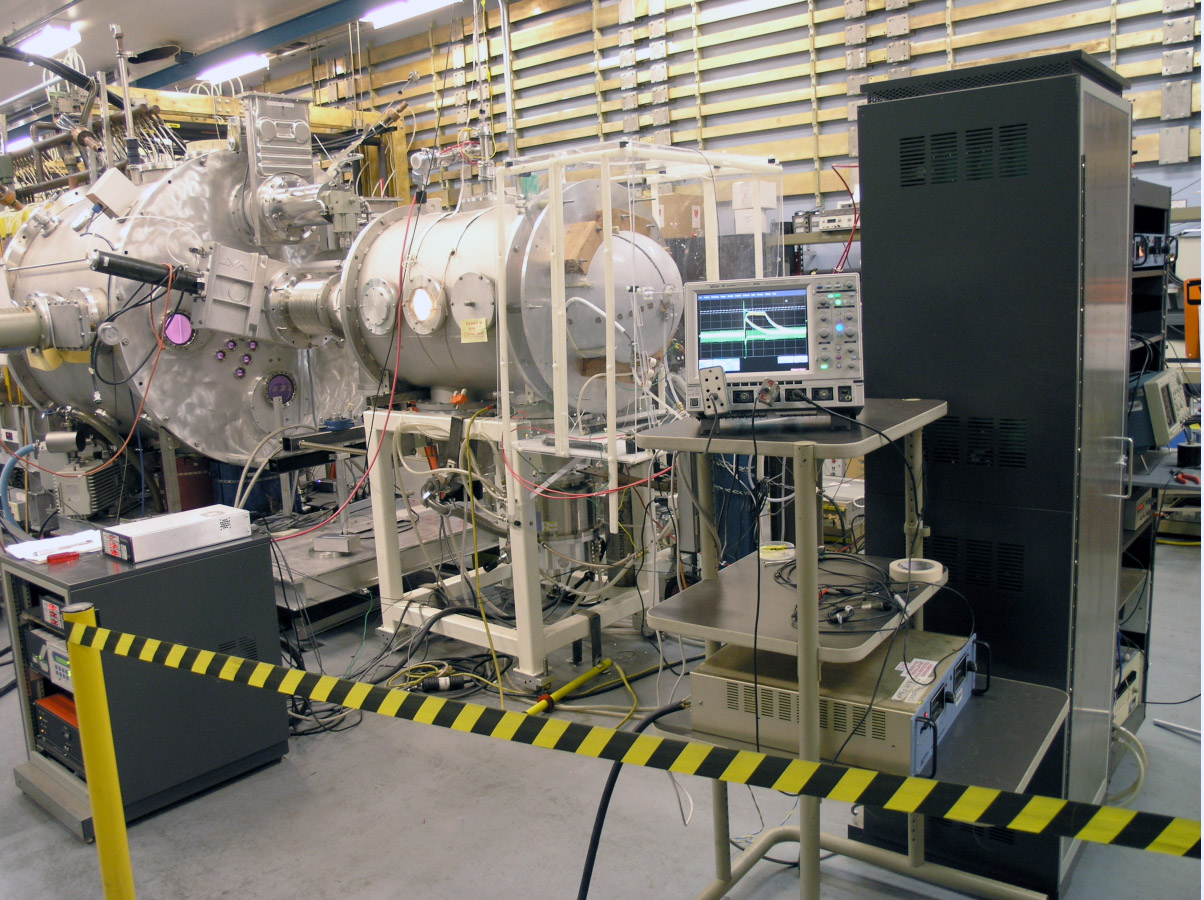
\includegraphics[width=0.95\textwidth]{ionbeamsource.jpg} 
   \caption{\small Ion beam attached to the end of the LAPD.  The beam is on a bellows and can be rotated about the center axis of the device, allowing injection at angles up to 15 degrees. The gate valve at the end allows the beam to be introduced without letting the machine up to air. }
   \label{fig:ionbeamsource}
\end{figure}
\begin{figure}[htbp] %  figure placement: here, top, bottom, or page
   \centering
   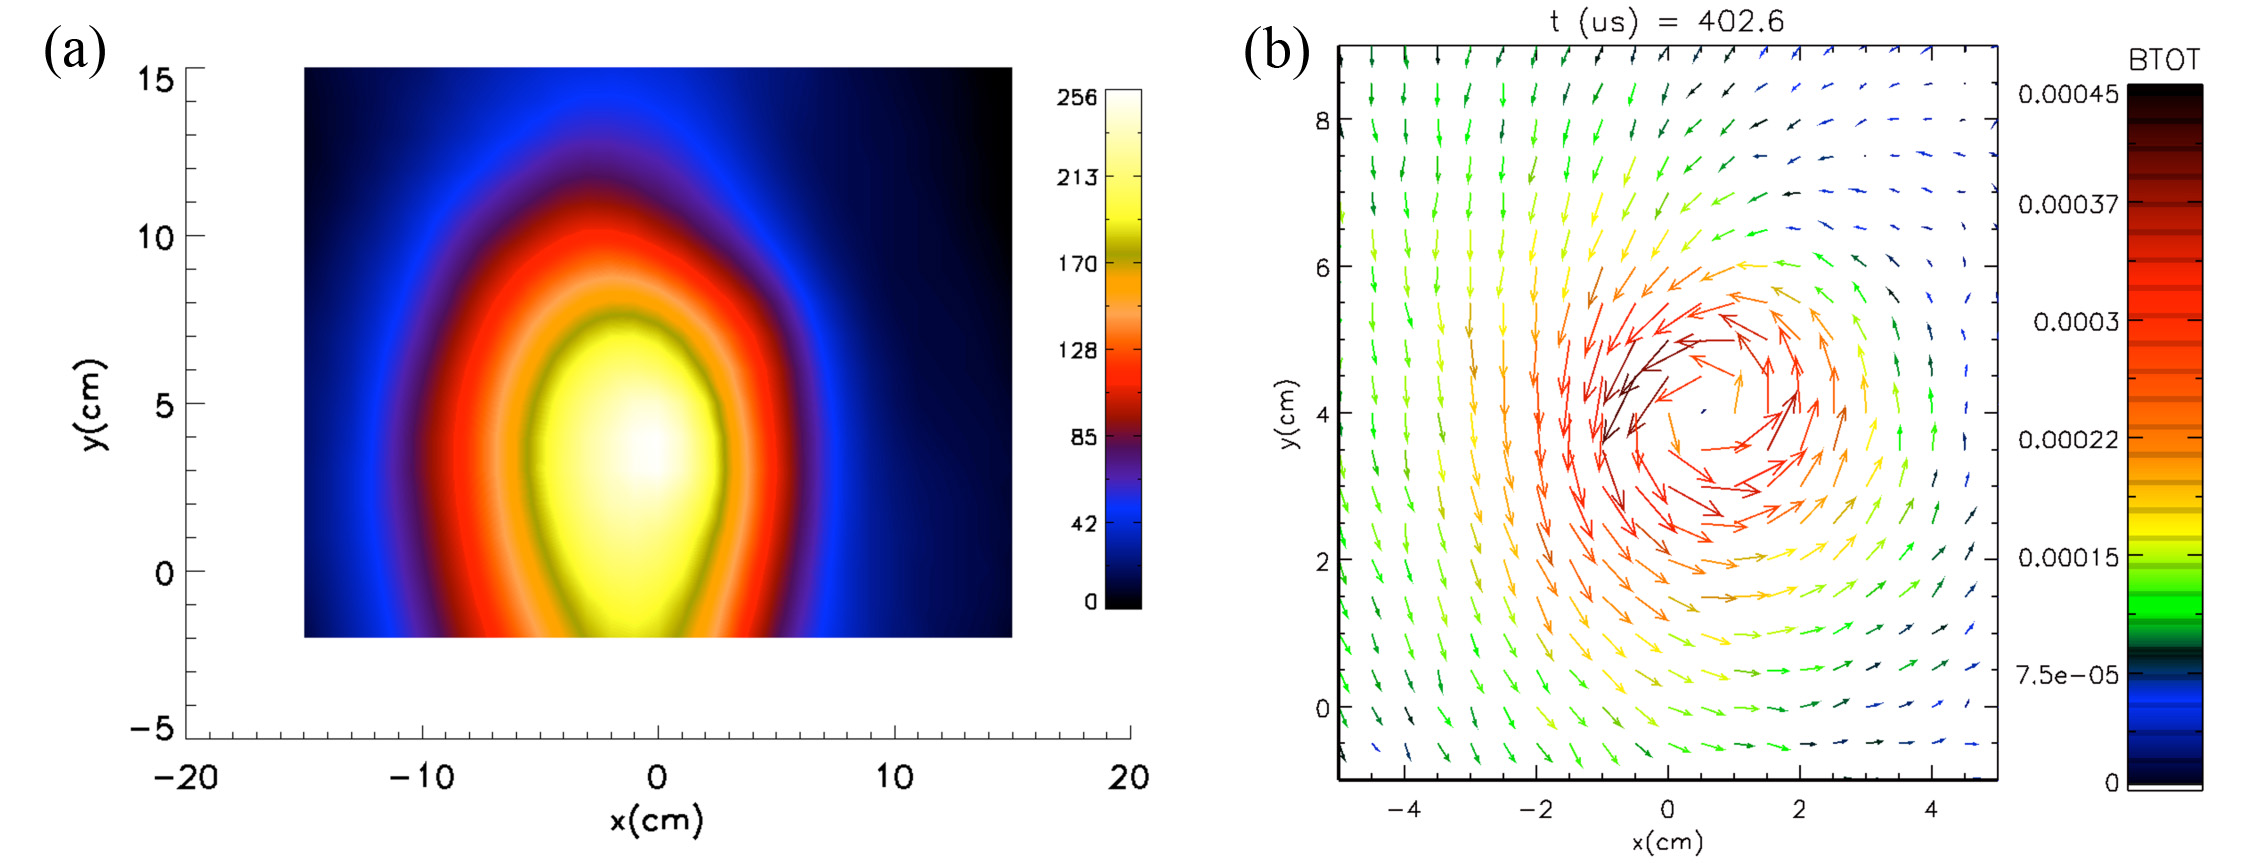
\includegraphics[width=0.95\textwidth]{ionbeam_and_wave.jpg} 
   \caption{\small (a) Helium ion beam ($V_{beam}$ = 22 keV) profile 4.28 m away from the beam source.  The brightest region corresponds to $n_{b} = 10^{8} $cm$^{-3}$. (b) Vector map of the fluctuating magnetic field excited by the ion beam .  Mode frequency is 510 kHz, ion cyclotron frequency 513 kHz.  $V_{beam} = 22$ keV, $I_{beam} = 0.42$ A, LAPD magnetic field is 1.35 kG, background plasma density $n = 1.8 \times 10^{12}$ cm$^{-3}$. }
   \label{fig:ionbeam_and_wave}
\end{figure}
 
%\newpage

%\setcounter{page}{1}

%\bibliographystyle{unsrtnat}
%\bibliographystyle{prsty}
%\bibliographystyle{unsrt}
%\bibliography{refs}  




\end{document}
